Deep generative models are currently the leading method for AMC \cite{yang2019deep}. However, a major problem with this method is controlling the generation process towards a given compositional goal. For example, controlling a model trained on classical piano pieces to compose a tense piece for a horror movie scene. Controlling emotions in AMC has been actively investigated in the field of \textit{affective algorithmic composition} \cite{williams2015investigating}. Therefore, this chapter presents a literature review of this field, including models to represent emotion and methods to control emotion in symbolic AMC systems. Given the similarity between text and music generation tasks, this chapter also covers NLP methods to control neural natural language models.
% Besides controlling emotions, the AMC research community has also been investigating how to control structural attributes (e.g. chord progression, melody contour, orchestration) of music with deep generative models. These methods are also discussed in this chapter.
% Once again, it is important to highlight that only  music generation methods are discussed in this chapter.

\section{Affective Algorithmic Composition}

\textit{Affective algorithmic composition} (AAC) is a research field concerned about controlling AMC methods to compose music that makes listeners perceive or feel a given target emotion \cite{williams2015investigating}. AAC is essential to a variety of applications, ranging from soundtrack generation \cite{williams2015dynamic} to sonification \cite{Chen2015} and music therapy \cite{miranda2011brain}. The AAC community has explored various methods to compose music with a target emotion algorithmically: expert systems \cite{williams2015dynamic}, evolutionary algorithms \cite{kim2004composing}, Markov chains \cite{monteith2010automatic}, deep learning \cite{madhok2018sentimozart}, among others. These methods have used different \textit{models of emotion}, but most of them are concerned with controlling \textit{perceived emotions} instead of \textit{felt emotions}. Therefore, they are normally evaluated with a listening test (i.e. user study) or a qualitative analysis of generated samples. This section introduces the most common models of emotion used in the AAC literature and the different approaches to control emotion in AMC. It also highlights the different methodologies used in the AAC literature to conduct the qualitative analysis and the listening tests.

\subsection{Models of Emotion}

The study of affective phenomena has a very dense literature with multiple alternative theories \cite{ekkekakis2013measurement}. This section does not aim to discuss all of them but to provide a definition of emotion that is useful for designing neural LMs for AAC.  According to \citet{williams2015investigating}, the literature concerning the affective response to musical stimuli defines emotion as a short-lived episode, usually evoked by an identifiable stimulus event that can further influence or direct perception and action. Williams et al. \cite{williams2015investigating} also differentiate emotion from affect and mood, which are longer experiences commonly caused by emotions.

There are two main types of models used to represent emotions: \emph{categorical} and \emph{dimensional} \cite{eerola2011comparison}. Categorical models use discrete labels to classify emotions. For example, Ekman's model \cite{ekman1992argument} divides human emotions into six basic categories: anger, disgust, fear, happiness, sadness, and surprise. This model builds on the assumption that an independent neural system subserves every discrete basic emotion \cite{eerola2011comparison}. Therefore, any other secondary emotion (e.g. rage, frustration, grief) can be derived from the basic ones. \citet{parrott2001emotions} proposed a similar model, but deriving a hierarchical structure with the following six basic emotions: love, joy, surprise, anger, sadness, and fear. These basic emotions are expanded into secondary emotions (e.g. passion, pleasure, envy), which in turn derive ternary emotions (e.g. compassion, frustration, guilt). Some emotions are more present in the music domain and are evoked more easily than others. For example, it is more common for a person to feel happiness instead of disgust while listening to music. The Geneva Emotion Music Scale (GEMS) \cite{zentner2008emotions} is a categorical model specifically created to capture the emotions that are evoked by music. GEMS divides the space of musical emotions into nine categories: wonder, transcendence, tenderness, nostalgia, peacefulness, energy, joyful activation, tension, and sadness. These nine emotions group a total of 45 specific labels.

Dimensional models represent emotions as a set of coordinates in a low-dimensional space. For example, \citet{russell1980circumplex} proposed a general-purpose dimensional model called \textit{circumplex}, which describes emotions using two orthogonal dimensions: valence and arousal. Instead of an independent neural system for every basic emotion, the circumplex model assumes that all emotions arise from two independent neurophysiological systems dedicated to the processing of valence (positive--negative) and arousal (mild--intense). Figure \ref{fig:circumplex} shows a graphical representation of the circumplex model. The \textit{vector model} \cite{bradley1992remembering} is another two-dimensional model based on valence and arousal. It represents emotions as vectors, where valence is a binary dimension (positive or negative) that defines the vector's direction and arousal is a continuous dimension that defines the vector's magnitude.

\begin{figure}[!h]
\centering
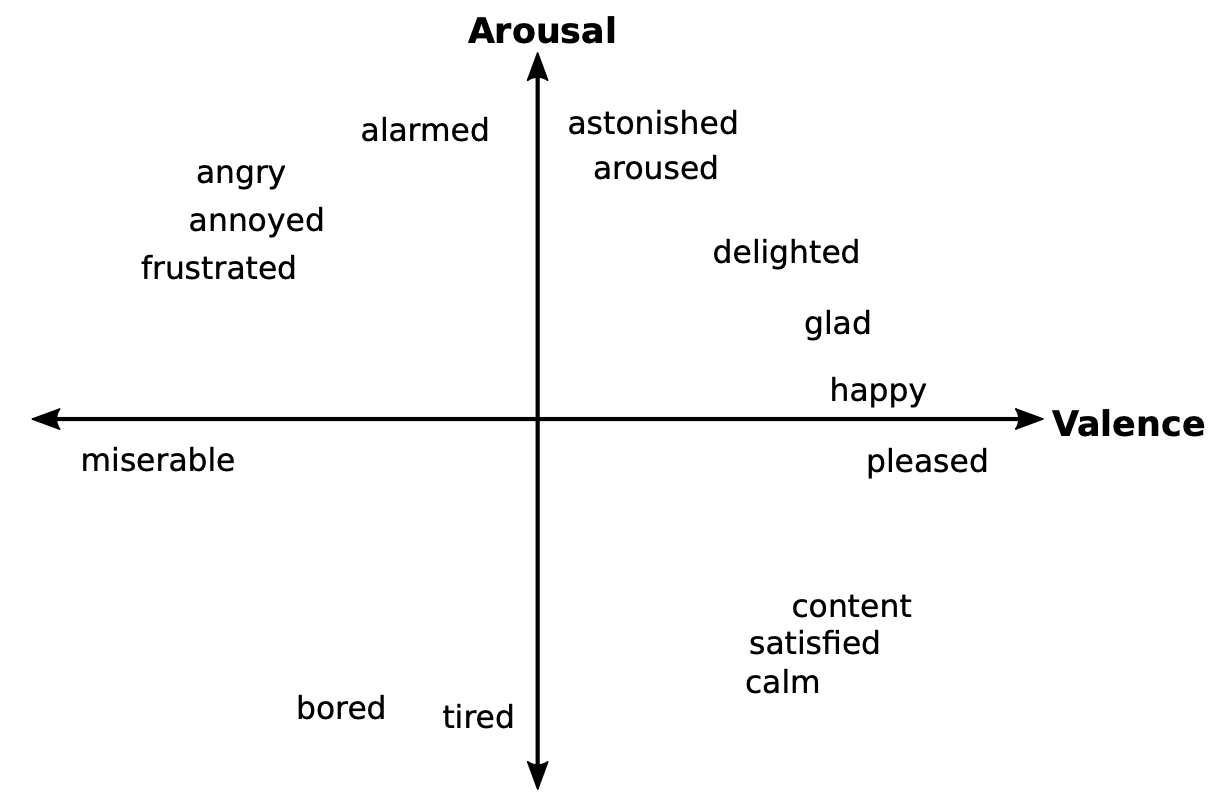
\includegraphics[width=0.7\textwidth]{imgs/related_work/circumplex.png}
\caption{The circumplex model of emotion. The horizontal and vertical axes represent valence and arousal,
respectively \cite{russell1980circumplex}.}
\label{fig:circumplex}
\end{figure}

Independent of the model, emotions can also be classified as \textit{perceived} or \textit{felt} \cite{gabrielsson2001emotion}. A person \textit{perceives} an emotion when they objectively recognize that emotion from their surroundings. For example, one can usually recognize someone else's emotion using expressed cues, including facial expression, tone of voice, and gestures. The same can happen when one listens to music, in that they recognize the music as happy or sad using cues such as key, tempo, or volume. A person \textit{feels} an emotion when they actually experience that emotion themselves. For example, one typically experiences fear in response to someone else's anger. This example shows that a given perceived emotion can trigger a different felt emotion. \citet{zentner2008emotions} showed that emotions are less frequently felt in response to music than perceived as expressive properties of the music.

\subsection{Expert systems}

Expert systems are one of the most common methods of AAC \cite{williams2015investigating}. They encode knowledge from music composers to map musical features into a given (categorical or dimensional) emotion. For example, \citet{williams2015dynamic} proposed a system to generate soundtracks for video games from a scene graph \footnote{A graph defining all the possible branching of scenes in the game.} annotated according to twelve categorical emotions derived from the circumplex model. First, a second-order Markov chain learns to generate melodies from a symbolic music dataset. Then, an expert system transforms the melodies generated via the Markov chain to match the annotated emotions in the graph. The transformations are performed by mapping each of the twelve emotions to a different configuration of five music parameters: rhythmic density, tempo, modality (major or minor), articulation, mean pitch range, and mean spectral range. For example, a melody generated for a happy scene would be transformed to have high density, medium tempo, major mode, staccato articulation, medium mean pitch range, and high spectral range (clear timbre). Williams et al. \cite{williams2015dynamic} evaluated their system by qualitatively examining a few examples of generated pieces.

TransProse \cite{davis2014generating} is an expert system that composes piano melodies for novels. It splits a given novel into sections and uses a lexicon-based approach to assign an emotion label to each section. TransProse composes a melody for each section by controlling the scale, tempo, octave, and notes of the melodies with pre-defined rules based on music theory. For example, the scale of a melody is determined by the sentiment of the section: positive sections are assigned a major scale, and negative sections are assigned a minor scale. TransProse was evaluated with a qualitative analysis of nine music pieces generated by the system for nine respective novels.

\citet{scirea2017affective} presented a framework called MetaCompose designed to create background music for games in real-time. MetaCompose generates music by (i) randomly creating a chord sequence from a pre-defined chord progression graph, (ii) evolving a melody for this chord sequence with a genetic algorithm and (iii) producing an accompaniment, adding rhythm and arpeggio, for the melody/harmony combination. Finally, MetaCompose uses an expert system called \textit{Real-Time Affective Music Composer} to transform the final composition to match a given emotion in the circumplex model. This expert system controls four musical attributes: volume, timbre, rhythm, dissonance. For example, low arousal pieces were controlled to have lower volume. Scirea et al. \cite{scirea2017affective} evaluated each component of the MetaCompose with a pairwise listening test. The components of the system were systematically (one-by-one) switched off and replaced with random generation, generating different ``broken'' versions of the framework. These broken versions were paired with the complete framework and evaluated by human subjects according to four criteria: pleasantness, randomness, harmoniousness, and interestingness. For each criteria, the participants were asked to prefer one of two pieces, also having the options of \textit{neither} and \textit{both equally}.

\subsection{Evolutionary Algorithms}

To control emotions in music generated with EAs, one has to define a fitness function that guides individuals encoding symbolic music towards a given emotion. It is very challenging to design a function that formally evaluates subjective aspects of music emotion. Thus, most EAs for AAC use interactive evaluation functions, where human subjects judge whether or not the generated pieces match a target emotion. The benefit of this approach is that when the population converges towards a target emotion, no further evaluation is needed to check if the generated pieces indeed match that emotion. However, every time one wants to generate a new set of pieces, the slow interactive evolutionary process
has to be restarted.

\citet{kim2004composing} proposed an IGA to compose polyrhythms\footnote{A polyrhythm is the concurrent playing of two or more different rhythms.} for four percussion instruments. It starts with a random population of polyrhythms and evolves them towards relaxing or disquieting emotions. A polyrhythm is encoded with four 16-bit strings, one for each instrument. A single bit in the string represents a beat division where 1 means that a (unpitched) note is played in that division and 0 means silence. The fitness of a polyrhythm is given by a human subject who judges it as relaxing, neutral, or disquieting. The selection strategy keeps the four most relaxing and four most disquieting individuals for reproduction with one-point crossover and mutation. Results showed that the genetic algorithm generated relaxing polyrhythms after 20 generations while it took only 10 for it to generate disquieting ones.

\citet{zhu2008emotional} presented an IGA based on the KTH rule system \cite{friberg2006overview} to create affective performances of pre-composed music pieces. The KTH rules model performance principles within the realm of Western classical, jazz and popular music. These rules control different music performance parameters (e.g. phrasing, articulation, tonal tension) with weights called \textit{k values} that represent the magnitude of each rule. Zhu et al. \cite{zhu2008emotional} encoded the individuals as a set of k values used to create MIDI performances of pre-composed pieces according to the KTH rules. The genetic algorithm evolves a population to find optimal k values that yield performances that are either happy or sad. The fitness of the performances are given by human subjects with a seven-point Likert scale.

\citet{nomura2018music} designed a distributed IGA to generate four-bar piano melodies with controllable ``brightness''. Multiple human evaluators evolve independent populations of melodies in parallel. In some generations, the genetic algorithm exchanges individuals between the independent populations. With the exchange, evaluators are affected by each other and the solutions are expected to agree with everyone's evaluations. Each individual in a population represents a melody with a sequence of sixteen pitch numbers (as defined by the MIDI protocol). Each element in the sequence is mapped into a quarter note with the pitch defined by the element. Evaluators give the fitness of an individual based on a seven-point Likert scale, where 1 means ``extremely dark'', 4 means ``neither'', and 7 means ``extremely bright''. An experiment with ten parallel evaluators showed that after seventeen generations, the independent populations converged to similar melodies.

\subsection{Markov Chains}

AAC systems based on Markov chains are typically hybrid systems where Markov chains compose an underlying piece of music that is transformed by an expert system. The work of \citet{williams2015dynamic} described earlier in this chapter is an example of such a system. Ramanto and Maulidevi \cite{ramanto2017markov} proposed a similar system in which the Markov chain is designed manually instead of derived from a corpus. There are not a lot of works training Markov chains directly from datasets of symbolic music labeled according to a model of emotion.

One of the few examples is the work of Monteith et al. \cite{monteith2010automatic, chan2008automatic}, which use different Markov models to generate polyphonic music from a MIDI corpus labeled according to the Parrott model of emotion \cite{parrott2001emotions}. The corpus is composed by 45 movie soundtracks labeled by 6 researchers using the 6 basic Parrott emotions: love, joy, surprise, anger, sadness, and fear. The system is divided into four main components: a rhythm generator, a pitch generator, a chord generator, and an instrumentation planner.
First, the rhythm generator randomly selects and transforms a rhythmic pattern from the subset of pieces with the target emotion. Second, the pitch generator assigns pitch values to the notes in the rhythm by sampling from a Markov chain trained with the pieces from the target emotion. Third, the chord generator generates an underlying harmony for the provided melody with a hidden Markov model. Finally, the instrumentation planner probabilistically selects the instruments for melodic and harmonic accompaniment based on the frequency of various melody and harmony instruments in the corpus.

The system uses single-layer feedforward networks, trained with the same MIDI corpus, to classify the outputs of the rhythm and melody generators as having the target emotion or not. The system only accepts rhythms and melodies classified by the neural networks as having the target emotion. Monteith et al. \cite{monteith2010automatic} evaluated their system with a listening test in which 13 human subjects selected the emotion that they perceived in the pieces. Moreover, the subjects used two 10-point Likert scales to evaluate how human-like and unique the pieces are.

% Chung and Vercoe \cite{chung2006affective} proposed a method to derive a Markov chain from physiological, physical, and self-reported data from listeners. They first composed original music pieces with different styles: jazz, jazz-funk, rock, electronic and dance music. Four audio clips were assembled for each of the five musical styles, providing 20 clips in total, each with a different level of vertical layering\footnote{The amount of musical layers stacked in a piece.} and horizontal complexity \footnote{The rhythmic complexity of a piece}.

\subsection{Deep Learning}

To train deep NNs that can generate music with a target emotion, one needs a relatively large dataset of symbolic music labeled according to a model of emotion. However, it is considerably expensive to create such a dataset because different people can perceive different emotions in the same piece. Thus, there is no single ground truth emotion label for a given piece. This subjectivity requires one to collect independent perceptions from different annotators in order to define a democratic ground truth label. The lack of labeled data is one of the reasons why deep learning approaches started being explored for AAC only recently. In fact, this dissertation is part of this early wave of works. The remainder of this section presents prominent deep learning approaches proposed to date. All of them use relatively small datasets and have been developed concurrently with this dissertation.

SentiMozart \cite{madhok2018sentimozart} is a framework that generates piano pieces that match the emotion of a given facial expression. It uses a convolutional NN to classify the emotion of a facial expression and an LSTM to generate a music piece corresponding to the identified emotion. The convolutional NN was trained with the FER-2013 \cite{goodfellow2013challenges} dataset, which has 35,887 images of facial expressions labeled with the following emotions: angry, disgust, fear, happy, sad, surprise, and neutral. To train the LSTM, \citet{madhok2018sentimozart} created a dataset with 200 MIDI piano pieces, each labeled by 15 annotators according to the classes happy, sad, and neutral. Three LSTM were trained independently, one for each emotion. To unify the models of emotion between the two datasets, \citet{madhok2018sentimozart} merged the categories sad, fear, angry, and disgust from the FER-2013 dataset into the sad emotion. The categories happy and surprise were mapped into the happy emotion. Thus, the output $e \in \{\textit{happy}, \textit{sad}, \textit{neutral}\}$ of the convolutional NN selects the respective LSTM that, in turn, composes a piece conveying the emotion $e$. SentiMozart was evaluated with a listening test where 30 human subjects judged 30 randomly chosen images (10 of each class) and their corresponding generated pieces. The participants used a 11-point Likert scale in which 0 means sad, 5 means neutral, and 10 means happy.

\citet{tan2020automated} proposed a deep NN for a similar problem: generating music that matches an emotion expressed by visual artworks (e.g. paintings, illustrations, collages). They paired images of paintings with MIDI piano pieces labeled with the same emotion and used an encoder-decoder network as a generative model. The encoder is a pre-trained convolutional NN called ResNet \cite{he2016deep}. \citet{tan2020automated} compared two decoders: an LSTM and a (decoder) transformer. The music pieces were encoded as sequences of tokens with the MIDI-based method proposed by \citet{oore2017learning}. \citet{tan2020automated} trained their model by pairing emotion-labeled images from \citet{you2016building} (17,349 images) with emotion-labeled music pieces from \citet{panda2013multi} (196 MIDI files). Since these two datasets use different categorical models of emotion, \citet{tan2020automated} mapped the emotion labels of the music dataset to the labels of the image dataset. The trained model was evaluated with a listening test and a machine classification test. In the listening test, six human subjects were asked to evaluate the sentiment of the music pieces and the images with a 10-point Likert scale without knowing which music piece was related to which image. The machine evaluation test consisted of training an emotional correspondence classifier to predict if a given pair of images and pieces express the same sentiment.

Zhao et al. \cite{zhao2019emotional} presented a conditional Biaxial LSTM \cite{johnson2017generating} to generate piano pieces with controllable emotion. They labeled the \textit{Piano midi.de} dataset according to a categorical model of emotion: happy, sad, peaceful, and tense. They used a piano roll representation for the input music pieces, which are processed by the LSTM together with an emotion signal associated with each time step of the input. This signal is encoded by an extra embedding layer and then added to the embedding of the input. Zhao et al. \cite{zhao2019emotional} evaluated the quality of the generated pieces according to four metrics of music structure: polyphony, scale consistency, 3-tone repetitions, and tone span. Moreover, they performed a listening test with 30 human subjects to evaluate if the subjects agree with the emotions intended by the model.

Music FaderNets \cite{tan2020music} is a framework based on a \textit{gaussian mixture variational autoencoder} (GM-VAE) that can learn high-level music feature representations (such as emotion) by modeling corresponding low-level structural music features. Based on \citet{yang2019deep}, Music FaderNets learns the low-level features of rhythm $z_r$, note density $z_d$, and key $z_k$ with separated RNN encoders $e_r$, $e_d$, and $e_k$, respectively. The high-level features are then inferred from the low-level representations ($z_r$, $z_d$, and $z_k$) via semisupervised clustering. Music Fadernets was trained to reconstruct pieces encoded as a sequence of tokens \cite{oore2017learning} extracted from the Yamaha Piano-e-Competition dataset \cite{yamahaEPiano} and the VGMIDI dataset\footnote{The VGMIDI dataset is a contribution of this dissertation described in Chaper \ref{ch:ismir19}.} \cite{ferreira_2019}. Results showed that Music Fadernets successfully learns the intrinsic relationship between arousal (high-level feature) and its corresponding low-level attributes of rhythm and note density.

% \section{Conditional Generative Models}

% Besides controlling emotion, the AMC community has also been investigating how to control general structural features in music. These methods typically are unsupervised approaches to learn disentangled representations of specific music features such as melody and rhythm. Such disentangled representations allows one to directly manipulate the output of the model. These approaches are related to this dissertation because one could use them to learn disentangled mappings between music structure and emotions. For example, EC2-VAE \cite{yang2019deep} is a VAE that learns disentangled representations of symbolic melodies, allowing the generation of melodies with controlled pitch contour and rhythm patterns. The encoder is a bidirectional GRU $E$ that maps the input melodies into a latent representation $z$. The decoder splits the latent representation $z$ to create two independent representations $z_p$ and $z_r$ for the pitch and the rhythm features of the melody, respectively. The rhythm representation $z_r$ is fed into a bidirectional GRU $D_r$ to reconstruct the rhythm of the melody. The output of $D_r$ is concatenated with $z_p$ and fed into another GRU $D_m$ to reconstruct the entire melody. Moreover, the EC2-VAE uses chords as a condition for both the encoder and decoder. EC2-VAE was trained with the Nottingham Dataset \cite{} to reconstruct entire melodies. The two independent decoder modules allows it to learn disentangled representations of pith and rhythm. Therefore, one can swap or interpolate the latent representations of different source melodies to compose new melodies that combine pitch and rhythm features from the source material.
%
% Music Sketchnet \cite{chen2020music} is a neural network \textit{music inpainting}\footnote{Music inpainting is the task of filling in missing or lost information in a piece of music.} framework that allows users to specify partial musical ideas guiding automatic music generation. Music Sketchnet is composed of three NN modules: SketchVAE, SketchInpainter, and SketchConnector. Similar to EC2-VAE \cite{yang2019deep}, SketchVAE \cite{chen2020music} is a VAE that creates independent representations of rhythm and pitch contour. SketchInpainter combines GRUs to perform the element-level inpainting prediction from the latent variables given by SketchVAE. SketchConnector uses a transformer NN to combined sketches of pitch and rhythm from users with the prediction from SketchInpainter and finalize the generation. Sketchnet was trained to reconstruct melodies from the Irish and Scottish monophonic music dataset \cite{}.

% Our work differs from these generative models because, instead of controlling structural music features, we control emotion which is a perceived feature that emerges from the music structure.

\section{Controllable Neural Language Models}
\label{sec:related_nlp}

Considering the similarities between music and natural LMs, this dissertation is also related to methods that control neural LMs to generate text with given characteristics (e.g. topic, style, sentiment). For example, \citet{radford_2017} showed that an LSTM can learn an excellent representation of sentiment (positive-negative) on text, despite being trained only to predict the next character in the Amazon reviews dataset \cite{He2016}. When fine-tuned with an extra linear layer, this LSTM achieved state-of-the-art sentiment analysis on the Stanford sentiment treebank dataset \cite{socher2013recursive}, matching the performance of previous supervised systems using 30-100x fewer labeled examples. \citet{radford_2017} observed that this LSTM stored almost all of the sentiment signal in a distinct \textit{sentiment neuron}, which could be used to control the LSTM to generate sentences with a given sentiment.

CTRL \cite{keskar2019ctrl} is a transformer LM trained to generate text conditioned on special tokens, called \textit{control codes}, that inform the LM about the characteristics (e.g. style) of the text to be generated. These control codes are derived automatically from the text source (e.g. Wikipedia), which means no manual annotation is needed. During training, every example sentence $x$ is processed together with a set of control codes. At generation time, CTRL can produce text with a particular style $s$, for example, by conditioning the prior input $x$ with a signal representing $s$.

% This dissertation differs from CTRL because we control the LM with a search procedure and not with an extra input to the LM. Conditioning the LM requires a large amount of labeled data, which is expensive in the affective music domain.

\citet{holtzman2018learning} proposed a decoding strategy that uses a set of discriminators (NNs) to steer the probability distribution of a LM at generation time. At each decoding step, the probabilities of the next words given by the LM are multiplied by weighted scores of four different discriminators: repetition, entailment, relevance, and lexical diversity. The discriminators are trained independently with a dataset of pairs $(x, y)$, where $x$ is a prior context sentence, and $y$ is the completion of that sentence. For each discriminator, the loss function measures the difference between the scores assigned to the truth continuation $y$ and the scores assigned to the continuation generated by the LM. Once all the discriminators are trained, Holtzman et al. \cite{holtzman2018learning} optimize the weights used to combine the score of each discriminator.

The Plug and Play LM \cite{dathathri2019plug} combines a pre-trained LM with an attribute (e.g. sentiment) classifier $C$ to guide text generation by fine-tuning the LM hidden layers at decoding time. At each generative time step, the LM hidden layers are shifted in the direction of the sum of two gradients: one towards the higher log-likelihood of the target attribute (as given by $C$) and the other towards higher log-likelihood of the unmodified LM. The shifting process occurs in three steps: (1) a forward pass using $C$ to compute the likelihood of the target attribute, (2) a backward pass to update the LM hidden states with gradients from the attribute classifier $C$, and (3) another forward pass to update the distribution over the vocabulary from the updated LM hidden layers. With this approach, multiple attribute classifiers can be combined at generation time with customized weights.

% Vijayakumar et al. \cite{vijayakumar2018diverse} and Kool et al. \cite{Kool2019SBS} proposed variations of beam search to solve the problem of generating repetitive sentences. Vijayakumar et al. \cite{vijayakumar2018diverse} decodes diverse lists by dividing candidate solutions into groups and enforcing diversity between groups. Kool et al. \cite{Kool2019SBS} applyes the ``Gumbel-Top-k'' trick to sample without replacement with beam search, mitigating the repetition problem. Our work differs from both these works because our variation of Beam search optimizes for two independent objectives.

% Ziegler et al. \cite{ziegler2019fine} used reinforcement learning to fine-tune a transformer LM for generating text with a given sentiment by using a reward model trained on human preferences on text continuations. They fine-tuned the model for two different tasks: generating text with sentiment and text summarization.
Given a music dataset labeled according to a model of emotion, one can apply the methods discussed in this section to control music LMs to generate pieces with a target emotion. The next chapter presents a method based on \citet{radford_2017} to control the sentiment of piano pieces generated by an LSTM. The chapter after that discusses a variation of beam-search inspired by \citet{holtzman2018learning} to control a transformer to generate piano pieces with a target emotion.
